% 若编译失败,且生成 .synctex(busy) 辅助文件,可能有两个原因:
% 1. 需要插入的图片不存在:Ctrl + F 搜索 'figure' 将这些代码注释/删除掉即可
% 2. 路径/文件名含中文或空格:更改路径/文件名即可

% ------------------------------------------------------------- %
% >> ------------------ 文章宏包及相关设置 ------------------ << %
% 设定文章类型与编码格式
\documentclass[UTF8]{report}		

% 本文特殊宏包
\usepackage{siunitx} % 埃米单位

% 本 .tex 专属的宏定义
    \def\V{\ \mathrm{V}}
    \def\mV{\ \mathrm{mV}}
    \def\kV{\ \mathrm{KV}}
    \def\KV{\ \mathrm{KV}}
    \def\MV{\ \mathrm{MV}}
    \def\A{\ \mathrm{A}}
    \def\mA{\ \mathrm{mA}}
    \def\kA{\ \mathrm{KA}}
    \def\KA{\ \mathrm{KA}}
    \def\MA{\ \mathrm{MA}}
    \def\O{\ \Omega}
    \def\mO{\ \Omega}
    \def\kO{\ \mathrm{K}\Omega}
    \def\KO{\ \mathrm{K}\Omega}
    \def\MO{\ \mathrm{M}\Omega}
    \def\Hz{\ \mathrm{Hz}}

% 自定义宏定义
    \def\N{\mathbb{N}}
    \def\F{\mathbb{F}}
    \def\Z{\mathbb{Z}}
    \def\Q{\mathbb{Q}}
    \def\R{\mathbb{R}}
    \def\C{\mathbb{C}}
    \def\T{\mathbb{T}}
    \def\S{\mathbb{S}}
    \def\A{\mathbb{A}}
    \def\I{\mathscr{I}}
    \def\Im{\mathrm{Im\,}}
    \def\Re{\mathrm{Re\,}}
    \def\d{\mathrm{d}}
    \def\p{\partial}

% 导入基本宏包
    \usepackage[UTF8]{ctex}     % 设置文档为中文语言
    \usepackage[colorlinks, linkcolor=blue, anchorcolor=blue, citecolor=blue, urlcolor=blue]{hyperref}  % 宏包:自动生成超链接 (此宏包与标题中的数学环境冲突)
    % \usepackage{hyperref}  % 宏包:自动生成超链接 (此宏包与标题中的数学环境冲突)
    % \hypersetup{
    %     colorlinks=true,    % false:边框链接 ; true:彩色链接
    %     citecolor={blue},    % 文献引用颜色
    %     linkcolor={blue},   % 目录 (我们在目录处单独设置),公式,图表,脚注等内部链接颜色
    %     urlcolor={orange},    % 网页 URL 链接颜色,包括 \href 中的 text
    %     % cyan 浅蓝色 
    %     % magenta 洋红色
    %     % yellow 黄色
    %     % black 黑色
    %     % white 白色
    %     % red 红色
    %     % green 绿色
    %     % blue 蓝色
    %     % gray 灰色
    %     % darkgray 深灰色
    %     % lightgray 浅灰色
    %     % brown 棕色
    %     % lime 石灰色
    %     % olive 橄榄色
    %     % orange 橙色
    %     % pink 粉红色
    %     % purple 紫色
    %     % teal 蓝绿色
    %     % violet 紫罗兰色
    % }

    % \usepackage{docmute}    % 宏包:子文件导入时自动去除导言区,用于主/子文件的写作方式,\include{./51单片机笔记}即可。注:启用此宏包会导致.tex文件capacity受限。
    \usepackage{amsmath}    % 宏包:数学公式
    \usepackage{mathrsfs}   % 宏包:提供更多数学符号
    \usepackage{amssymb}    % 宏包:提供更多数学符号
    \usepackage{pifont}     % 宏包:提供了特殊符号和字体
    \usepackage{extarrows}  % 宏包:更多箭头符号
    \usepackage{multicol}   % 宏包:支持多栏 
    \usepackage{graphicx}   % 宏包:插入图片
    \usepackage{float}      % 宏包:设置图片浮动位置
    %\usepackage{article}    % 宏包:使文本排版更加优美
    \usepackage{tikz}       % 宏包:绘图工具
    %\usepackage{pgfplots}   % 宏包:绘图工具
    \usepackage{enumerate}  % 宏包:列表环境设置
    \usepackage{enumitem}   % 宏包:列表环境设置

% 文章页面margin设置
    \usepackage[a4paper]{geometry}
        \geometry{top=1in}
        \geometry{bottom=1in}
        \geometry{left=0.75in}
        \geometry{right=0.75in}   % 设置上下左右页边距
        \geometry{marginparwidth=1.75cm}    % 设置边注距离(注释、标记等)

% 定义 solution 环境
\usepackage{amsthm}
\newtheorem{solution}{Solution}
        \geometry{bottom=1in}
        \geometry{left=0.75in}
        \geometry{right=0.75in}   % 设置上下左右页边距
        \geometry{marginparwidth=1.75cm}    % 设置边注距离(注释、标记等)

% 配置数学环境
    \usepackage{amsthm} % 宏包:数学环境配置
    % theorem-line 环境自定义
        \newtheoremstyle{MyLineTheoremStyle}% <name>
            {11pt}% <space above>
            {11pt}% <space below>
            {}% <body font> 使用默认正文字体
            {}% <indent amount>
            {\bfseries}% <theorem head font> 设置标题项为加粗
            {:}% <punctuation after theorem head>
            {.5em}% <space after theorem head>
            {\textbf{#1}\thmnumber{#2}\ \ (\,\textbf{#3}\,)}% 设置标题内容顺序
        \theoremstyle{MyLineTheoremStyle} % 应用自定义的定理样式
        \newtheorem{LineTheorem}{Theorem.\,}
    % theorem-block 环境自定义
        \newtheoremstyle{MyBlockTheoremStyle}% <name>
            {11pt}% <space above>
            {11pt}% <space below>
            {}% <body font> 使用默认正文字体
            {}% <indent amount>
            {\bfseries}% <theorem head font> 设置标题项为加粗
            {:\\ \indent}% <punctuation after theorem head>
            {.5em}% <space after theorem head>
            {\textbf{#1}\thmnumber{#2}\ \ (\,\textbf{#3}\,)}% 设置标题内容顺序
        \theoremstyle{MyBlockTheoremStyle} % 应用自定义的定理样式
        \newtheorem{BlockTheorem}[LineTheorem]{Theorem.\,} % 使用 LineTheorem 的计数器
    % definition 环境自定义
        \newtheoremstyle{MySubsubsectionStyle}% <name>
            {11pt}% <space above>
            {11pt}% <space below>
            {}% <body font> 使用默认正文字体
            {}% <indent amount>
            {\bfseries}% <theorem head font> 设置标题项为加粗
           % {:\\ \indent}% <punctuation after theorem head>
            {\\\indent}
            {0pt}% <space after theorem head>
            {\textbf{#3}}% 设置标题内容顺序
        \theoremstyle{MySubsubsectionStyle} % 应用自定义的定理样式
        \newtheorem{definition}{}

%宏包:有色文本框(proof环境)及其设置
    \usepackage[dvipsnames,svgnames]{xcolor}    %设置插入的文本框颜色
    \usepackage[strict]{changepage}     % 提供一个 adjustwidth 环境
    \usepackage{framed}     % 实现方框效果
        \definecolor{graybox_color}{rgb}{0.95,0.95,0.96} % 文本框颜色。修改此行中的 rgb 数值即可改变方框纹颜色,具体颜色的rgb数值可以在网站https://colordrop.io/ 中获得。(截止目前的尝试还没有成功过,感觉单位不一样)(找到喜欢的颜色,点击下方的小眼睛,找到rgb值,复制修改即可)
        \newenvironment{graybox}{%
        \def\FrameCommand{%
        \hspace{1pt}%
        {\color{gray}\small \vrule width 2pt}%
        {\color{graybox_color}\vrule width 4pt}%
        \colorbox{graybox_color}%
        }%
        \MakeFramed{\advance\hsize-\width\FrameRestore}%
        \noindent\hspace{-4.55pt}% disable indenting first paragraph
        \begin{adjustwidth}{}{7pt}%
        \vspace{2pt}\vspace{2pt}%
        }
        {%
        \vspace{2pt}\end{adjustwidth}\endMakeFramed%
        }



% 外源代码插入设置
    % matlab 代码插入设置
    \usepackage{matlab-prettifier}
        \lstset{style=Matlab-editor}    % 继承 matlab 代码高亮 , 此行不能删去
    \usepackage[most]{tcolorbox} % 引入tcolorbox包 
    \usepackage{listings} % 引入listings包
        \tcbuselibrary{listings, skins, breakable}
        \newfontfamily\codefont{Consolas} % 定义需要的 codefont 字体
        \lstdefinestyle{MatlabStyle_inc}{   % 插入代码的样式
            language=Matlab,
            basicstyle=\small\ttfamily\codefont,    % ttfamily 确保等宽 
            breakatwhitespace=false,
            breaklines=true,
            captionpos=b,
            keepspaces=true,
            numbers=left,
            numbersep=15pt,
            showspaces=false,
            showstringspaces=false,
            showtabs=false,
            tabsize=2,
            xleftmargin=15pt,   % 左边距
            %frame=single, % single 为包围式单线框
            frame=shadowbox,    % shadowbox 为带阴影包围式单线框效果
            %escapeinside=``,   % 允许在代码块中使用 LaTeX 命令 (此行无用)
            %frameround=tttt,    % tttt 表示四个角都是圆角
            framextopmargin=0pt,    % 边框上边距
            framexbottommargin=0pt, % 边框下边距
            framexleftmargin=5pt,   % 边框左边距
            framexrightmargin=5pt,  % 边框右边距
            rulesepcolor=\color{red!20!green!20!blue!20}, % 阴影框颜色设置
            %backgroundcolor=\color{blue!10}, % 背景颜色
        }
        \lstdefinestyle{MatlabStyle_src}{   % 插入代码的样式
            language=Matlab,
            basicstyle=\small\ttfamily\codefont,    % ttfamily 确保等宽 
            breakatwhitespace=false,
            breaklines=true,
            captionpos=b,
            keepspaces=true,
            numbers=left,
            numbersep=15pt,
            showspaces=false,
            showstringspaces=false,
            showtabs=false,
            tabsize=2,
        }
        \newtcblisting{matlablisting}{
            %arc=2pt,        % 圆角半径
            % 调整代码在 listing 中的位置以和引入文件时的格式相同
            top=0pt,
            bottom=0pt,
            left=-5pt,
            right=-5pt,
            listing only,   % 此句不能删去
            listing style=MatlabStyle_src,
            breakable,
            colback=white,   % 选一个合适的颜色
            colframe=black!0,   % 感叹号后跟不透明度 (为 0 时完全透明)
        }
        \lstset{
            style=MatlabStyle_inc,
        }



% table 支持
    \usepackage{booktabs}   % 宏包:三线表
    %\usepackage{tabularray} % 宏包:表格排版
    %\usepackage{longtable}  % 宏包:长表格
    %\usepackage[longtable]{multirow} % 宏包:multi 行列


% figure 设置
\usepackage{graphicx}   % 支持 jpg, png, eps, pdf 图片 
\usepackage{float}      % 支持 H 选项
\usepackage{svg}        % 支持 svg 图片
\usepackage{subcaption} % 支持子图
\svgsetup{
        % 指向 inkscape.exe 的路径
       inkscapeexe = C:/aa_MySame/inkscape/bin/inkscape.exe, 
        % 一定程度上修复导入后图片文字溢出几何图形的问题
       inkscapelatex = false                 
   }

% 图表进阶设置
    \usepackage{caption}    % 图注、表注
        \captionsetup[figure]{name=图}  
        \captionsetup[table]{name=表}
        \captionsetup{
            labelfont=bf, % 设置标签为粗体
            textfont=bf,  % 设置文本为粗体
            font=small  
        }
    \usepackage{float}     % 图表位置浮动设置 
        % \floatstyle{plaintop} % 设置表格标题在表格上方
        % \restylefloat{table}  % 应用设置


% 圆圈序号自定义
    \newcommand*\circled[1]{\tikz[baseline=(char.base)]{\node[shape=circle,draw,inner sep=0.8pt, line width = 0.03em] (char) {\small \bfseries #1};}}   % TikZ solution


% 列表设置
    \usepackage{enumitem}   % 宏包:列表环境设置
        \setlist[enumerate]{
            label=\bfseries(\arabic*) ,   % 设置序号样式为加粗的 (1) (2) (3)
            ref=\arabic*, % 如果需要引用列表项,这将决定引用格式(这里仍然使用数字)
            itemsep=0pt, parsep=0pt, topsep=0pt, partopsep=0pt, leftmargin=3.5em} 
        \setlist[itemize]{itemsep=0pt, parsep=0pt, topsep=0pt, partopsep=0pt, leftmargin=3.5em}
        \newlist{circledenum}{enumerate}{1} % 创建一个新的枚举环境  
        \setlist[circledenum,1]{  
            label=\protect\circled{\arabic*}, % 使用 \arabic* 来获取当前枚举计数器的值,并用 \circled 包装它  
            ref=\arabic*, % 如果需要引用列表项,这将决定引用格式(这里仍然使用数字)
            itemsep=0pt, parsep=0pt, topsep=0pt, partopsep=0pt, leftmargin=3.5em
        }  

% 文章默认字体设置
    \usepackage{fontspec}   % 宏包:字体设置
        \setmainfont{STKaiti}    % 设置中文字体为宋体字体
        \setCJKmainfont[AutoFakeBold=3]{STKaiti} % 设置加粗字体为 STKaiti 族,AutoFakeBold 可以调整字体粗细
        \setmainfont{Times New Roman} % 设置英文字体为Times New Roman


% 其它设置
    % 脚注设置
    \renewcommand\thefootnote{\ding{\numexpr171+\value{footnote}}}
    % 参考文献引用设置
        \bibliographystyle{unsrt}   % 设置参考文献引用格式为unsrt
        \newcommand{\upcite}[1]{\textsuperscript{\cite{#1}}}     % 自定义上角标式引用
    % 文章序言设置
        \newcommand{\cnabstractname}{序言}
        \newenvironment{cnabstract}{%
            \par\Large
            \noindent\mbox{}\hfill{\bfseries \cnabstractname}\hfill\mbox{}\par
            \vskip 2.5ex
            }{\par\vskip 2.5ex}


% 各级标题自定义设置
    \usepackage{titlesec}   
    % chapter
        \titleformat{\chapter}[hang]{\normalfont\Large\bfseries\centering}{题目}{10pt}{}
        \titlespacing*{\chapter}{0pt}{-30pt}{10pt} % 控制上方空白的大小
    % section
        \titleformat{\section}[hang]{\normalfont\large\bfseries}{\thesection}{8pt}{}
    % subsection
        %\titleformat{\subsubsection}[hang]{\normalfont\bfseries}{}{8pt}{}
    % subsubsection
        %\titleformat{\subsubsection}[hang]{\normalfont\bfseries}{}{8pt}{}

% 见到的一个有意思的对于公式中符号的彩色解释的环境
        \usepackage[dvipsnames]{xcolor}
        \usepackage{tikz}
        \usetikzlibrary{backgrounds}
        \usetikzlibrary{arrows,shapes}
        \usetikzlibrary{tikzmark}
        \usetikzlibrary{calc}
        
        \usepackage{amsmath}
        \usepackage{amsthm}
        \usepackage{amssymb}
        \usepackage{mathtools, nccmath}
        \usepackage{wrapfig}
        \usepackage{comment}
        
        % To generate dummy text
        \usepackage{blindtext}
        
        
        %color
        %\usepackage[dvipsnames]{xcolor}
        % \usepackage{xcolor}
        
        
        %\usepackage[pdftex]{graphicx}
        \usepackage{graphicx}
        % declare the path(s) for graphic files
        %\graphicspath{{../Figures/}}
        
        % extensions so you won't have to specify these with
        % every instance of \includegraphics
        % \DeclareGraphicsExtensions{.pdf,.jpeg,.png}
        
        % for custom commands
        \usepackage{xspace}
        
        % table alignment
        \usepackage{array}
        \usepackage{ragged2e}
        \newcolumntype{P}[1]{>{\RaggedRight\hspace{0pt}}p{#1}}
        \newcolumntype{X}[1]{>{\RaggedRight\hspace*{0pt}}p{#1}}
        
        % color box
        \usepackage{tcolorbox}
        
        
        % for tikz
        \usepackage{tikz}
        %\usetikzlibrary{trees}
        \usetikzlibrary{arrows,shapes,positioning,shadows,trees,mindmap}
        \usetikzlibrary{graphs} % <-- Added for \graph syntax
        % \usepackage{forest}
        \usepackage[edges]{forest}
        \usetikzlibrary{arrows.meta}
        \colorlet{linecol}{black!75}
        \usepackage{xkcdcolors} % xkcd colors
        
        
        % for colorful equation
        \usepackage{tikz}
        \usetikzlibrary{backgrounds}
        \usetikzlibrary{arrows,shapes}
        \usetikzlibrary{tikzmark}
        \usetikzlibrary{calc}
        % Commands for Highlighting text -- non tikz method
        \newcommand{\highlight}[2]{\colorbox{#1!17}{$\displaystyle #2$}}
        %\newcommand{\highlight}[2]{\colorbox{#1!17}{$#2$}}
        \newcommand{\highlightdark}[2]{\colorbox{#1!47}{$\displaystyle #2$}}
        
        % my custom colors for shading
        \colorlet{mhpurple}{Plum!80}
        
        
        % Commands for Highlighting text -- non tikz method
        \renewcommand{\highlight}[2]{\colorbox{#1!17}{#2}}
        \renewcommand{\highlightdark}[2]{\colorbox{#1!47}{#2}}
        
        % Some math definitions
        \newcommand{\lap}{\mathrm{Lap}}
        \newcommand{\pr}{\mathrm{Pr}}
        
        \newcommand{\Tset}{\mathcal{T}}
        \newcommand{\Dset}{\mathcal{D}}
        \newcommand{\Rbound}{\widetilde{\mathcal{R}}}

% >> ------------------ 文章宏包及相关设置 ------------------ << %
% ------------------------------------------------------------- %



% ----------------------------------------------------------- %
% >> --------------------- 文章信息区 --------------------- << %
% 页眉页脚设置

\usepackage{fancyhdr}   %宏包:页眉页脚设置
    \pagestyle{fancy}
    \fancyhf{}
    \cfoot{\thepage}
    \renewcommand\headrulewidth{1pt}
    \renewcommand\footrulewidth{0pt}
    \rhead{数据结构与算法期末复习,\ 尹超,\ 2023K8009926003}
    \lhead{Homework}


%文档信息设置
\title{数据结构与算法期末复习\\ Homework}
\author{尹超\\ \footnotesize 中国科学院大学,北京 100049\\ Carter Yin \\ \footnotesize University of Chinese Academy of Sciences, Beijing 100049, China}
\date{\footnotesize 2024.8 -- 2025.1}
% >> --------------------- 文章信息区 --------------------- << %
% ----------------------------------------------------------- %     


% 开始编辑文章

% 定义 tikz 样式 splaynode 和 highlight
\tikzset{
  splaynode/.style={draw, circle, minimum size=7mm, inner sep=0pt},
  highlight/.style={draw, circle, minimum size=7mm, inner sep=0pt, fill=yellow!30}
}

\begin{document}
\zihao{5}           % 设置全文字号大小

% --------------------------------------------------------------- %
% >> --------------------- 封面序言与目录 --------------------- << %
% 封面
    \maketitle\newpage  
    \pagenumbering{Roman} % 页码为大写罗马数字
    \thispagestyle{fancy}   % 显示页码、页眉等

% 序言
    \begin{cnabstract}\normalsize 
        本文为笔者数据结构与算法的期末复习笔记。\par
        望老师批评指正。
    \end{cnabstract}
    \addcontentsline{toc}{chapter}{序言} % 手动添加为目录

% % 不换页目录
%     \setcounter{tocdepth}{0}
%     \noindent\rule{\textwidth}{0.1em}   % 分割线
%     \noindent\begin{minipage}{\textwidth}\centering 
%         \vspace{1cm}
%         \tableofcontents\thispagestyle{fancy}   % 显示页码、页眉等   
%     \end{minipage}  
%     \addcontentsline{toc}{chapter}{目录} % 手动添加为目录

% 目录
\setcounter{tocdepth}{4}                % 目录深度(为1时显示到section)
\tableofcontents                        % 目录页
\addcontentsline{toc}{chapter}{目录}    % 手动添加此页为目录
\thispagestyle{fancy}                   % 显示页码、页眉等 

% 收尾工作
    \newpage    
    \pagenumbering{arabic} 

% >> --------------------- 封面序言与目录 --------------------- << %
% --------------------------------------------------------------- %

\chapter{第十章 图应用}

\section*{169}
\begin{graybox}
如果把朋友圈视为一无向图,那么即使A君看
不到你给B点的赞,你们仍可能属于同一双连通分
量。
\end{graybox}

\begin{solution}
这个说法是\textbf{正确}的。

\textbf{详细分析:}

\begin{enumerate}
    \item \textbf{图模型解释:}
    \begin{itemize}
        \item \textbf{朋友圈 = 无向图}: 每个用户是一个顶点,好友关系是一条无向边。
        \item \textbf{A君看不到你的赞}: 这通常意味着你和A君不是直接好友。在图模型中,即顶点“你”和顶点“A”之间没有直接的边。
        \item \textbf{双连通分量 (Biconnected Component)}: 这是图的一个子图,其中任意两个顶点之间都至少存在两条\textbf{顶点不相交}的路径。通俗地讲,这意味着移除分量中的任意一个“中间人”(顶点),你和A君之间仍然是连通的。这是一种非常“紧密”和“鲁棒”的社群结构。
    \end{itemize}

    \item \textbf{举例说明:}
    你和A君不直接是好友,但你们有两个或更多的共同好友。例如,C和D。
    \begin{itemize}
        \item 你是C的好友,A也是C的好友。
        \item 你是D的好友,A也是D的好友。
    \end{itemize}
    这就构成了一个环路:你 -- C -- A -- D -- 你。

    \begin{center}
    \begin{tikzpicture}[
        node distance=2cm,
        every node/.style={circle, draw, font=\sffamily\bfseries, minimum size=1cm}
    ]
        \node (You) {你};
        \node (C) [above right=of You] {C};
        \node (D) [below right=of You] {D};
        \node (A) [right=of C] {A};
        
        \path[draw, thick, <->]
            (You) edge node[above, sloped] {好友} (C)
            (You) edge node[below, sloped] {好友} (D)
            (C) edge node[above, sloped] {好友} (A)
            (D) edge node[below, sloped] {好友} (A);
    \end{tikzpicture}
    \end{center}

    在这个结构中:
    \begin{itemize}
        \item 你和A之间没有直接的边。
        \item 存在路径1:你 $\to$ C $\to$ A。
        \item 存在路径2:你 $\to$ D $\to$ A。
    \end{itemize}
    这两条路径除了起点(你)和终点(A)之外,没有任何共同的顶点。因此,你和A处于同一个双连通分量中。即使你们的共同好友C(或D)注销了账号,你们依然可以通过另一位共同好友D(或C)保持联系。
\end{enumerate}

\textbf{结论:}
没有直接联系(边)并不妨碍两个顶点同属于一个双连通分量。只要它们之间存在至少两条独立的路径,它们的关系就是双连通的。
\end{solution}

\section*{170}
\begin{graybox}
对于同一无向图,起始于顶点s的DFS尽
管可能得到结构不同的DFS树,但s在树中的度
数必然固定。
\end{graybox}

\begin{solution}
这个说法是\textbf{正确}的。

\textbf{详细分析:}

\begin{enumerate}
    \item \textbf{DFS树中顶点的度:}
    在DFS树中,一个顶点 `u` 的度数等于它作为父节点所拥有的子节点数量。一个邻居 `v` 成为 `u` 的子节点,当且仅当DFS通过边 `(u, v)` 第一次访问到 `v` 时(即 `v` 尚未被访问过)。

    \item \textbf{关键思想:邻居的连通性}
    \begin{itemize}
        \item 设 `s` 在原图中的所有邻居构成集合 `N(s)`。
        \item 考虑将顶点 `s` 从原图中移除后,由 `N(s)` 中的顶点所构成的子图。这个子图可能会被分为一个或多个连通分量。
        \item 当DFS从 `s` 开始,并选择其第一个邻居(比如 `$v_1$`)进行深入访问时,这次递归调用将会访问到与 `$v_1$` 在 `N(s)` 的子图中属于同一个连通分量的所有其他邻居。
        \item 因此,当DFS从 `$v_1$` 的递归中返回到 `s` 时,`s` 再去检查 `N(s)` 中与 `$v_1$` 属于同一连通分量的其他邻居时,会发现它们都已经被访问过了,于是不会再与它们形成树边。
    \end{itemize}

    \item \textbf{结论:}
    `s` 在DFS树中的度数,精确地等于 **`s` 的邻居集 `N(s)` 在移除 `s` 后的子图中所形成的连通分量的数量**。
    这个数量是一个图的结构性属性,它不随DFS遍历邻居的顺序而改变。因此,无论DFS树的结构如何变化,`s` 在树中的度数是固定的。

    \item \textbf{示例:}
    考虑一个环 `s-a-b-c-s`。
    \begin{center}
    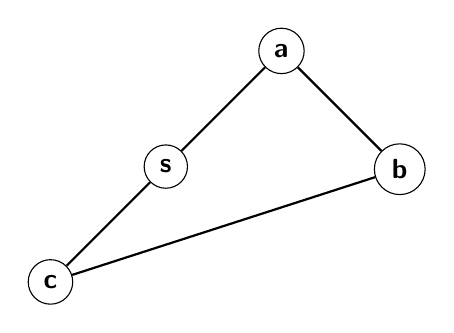
\begin{tikzpicture}[
        node distance=1.5cm,
        every node/.style={circle, draw, font=\sffamily\bfseries}
    ]
        \node (s) {s};
        \node (a) [above right=of s] {a};
        \node (b) [below right=of a] {b};
        \node (c) [below left=of s] {c};
        
        \path[draw, thick]
            (s) edge (a)
            (a) edge (b)
            (b) edge (c)
            (c) edge (s);
    \end{tikzpicture}
    \end{center}
    \begin{itemize}
        \item `s` 的邻居是 `a` 和 `c`。
        \item 移除 `s` 后,`a` 和 `c` 通过路径 `a-b-c` 仍然是连通的。它们属于同一个连通分量。
        \item 因此,`s` 在DFS树中的度数必然是1。
        \item \textbf{验证:}
            \begin{itemize}
                \item 若先访问 `a`:DFS路径为 `s->a->b->c`。`c` 被访问后,返回到 `s` 时发现 `c` 已被访问。`s` 的孩子只有 `a`,度为1。
                \item 若先访问 `c`:DFS路径为 `s->c->b->a`。`a` 被访问后,返回到 `s` 时发现 `a` 已被访问。`s` 的孩子只有 `c`,度为1。
            \end{itemize}
    \end{itemize}
\end{enumerate}
\end{solution}



\section*{171}
\begin{graybox}
已知有向图G=(V, E),其中V = \{v1, v2,v3, v4, v5, v6\},\\
E = \{<v1,v2>, <v1,v4>,<v2,v6>, <v3,v1>, <v3,v4>, <v4,v5>,<v5,v2>, <v5,v6>\}。\\
G的拓扑序列是:\\
A. v1, v3, v4, v5, v2, v6\\
B. v3, v4, v1, v5, v2, v6\\
C. v1, v4, v3, v5, v2, v6\\
D. v3, v1, v4, v5, v2, v6\\
\end{graybox}

\begin{solution}
正确答案是 D。

\textbf{详细分析:}

拓扑排序的核心规则是:对于图中的任意一条有向边 `<u, v>`,顶点 `u` 必须出现在顶点 `v` 之前。我们可以逐一检查每个选项是否违反了这个规则。

图中的边为:
\begin{itemize}
    \item <v1,v2>, <v1,v4>
    \item <v2,v6>
    \item <v3,v1>, <v3,v4>
    \item <v4,v5>
    \item <v5,v2>, <v5,v6>
\end{itemize}

\textbf{检查各个选项:}
\begin{itemize}
    \item \textbf{A. v1, v3, v4, v5, v2, v6} \\
    检查边 `<v3, v1>`。在这个序列中,`v3` 出现在 `v1` 之后,违反了规则。因此A是错误的。

    \item \textbf{B. v3, v4, v1, v5, v2, v6} \\
    检查边 `<v1, v4>`。在这个序列中,`v1` 出现在 `v4` 之后,违反了规则。因此B是错误的。

    \item \textbf{C. v1, v4, v3, v5, v2, v6} \\
    检查边 `<v3, v1>`。在这个序列中,`v3` 出现在 `v1` 之后,违反了规则。因此C是错误的。

    \item \textbf{D. v3, v1, v4, v5, v2, v6} \\
    我们来检查所有边:
    \begin{itemize}
        \item `<v1,v2>`: v1 在 v2 之前,正确。
        \item `<v1,v4>`: v1 在 v4 之前,正确。
        \item `<v2,v6>`: v2 在 v6 之前,正确。
        \item `<v3,v1>`: v3 在 v1 之前,正确。
        \item `<v3,v4>`: v3 在 v4 之前,正确。
        \item `<v4,v5>`: v4 在 v5 之前,正确。
        \item `<v5,v2>`: v5 在 v2 之前,正确。
        \item `<v5,v6>`: v5 在 v6 之前,正确。
    \end{itemize}
    所有边的约束都得到了满足。因此D是一个正确的拓扑序列。
\end{itemize}

\textbf{另一种方法:使用Kahn算法(基于入度)}
\begin{enumerate}
    \item 计算所有顶点的入度:
    in(v1)=1, in(v2)=2, in(v3)=0, in(v4)=2, in(v5)=1, in(v6)=2。
    \item 将所有入度为0的顶点(只有v3)放入队列。队列:`[v3]`。
    \item 从队列中取出v3,加入拓扑序列。序列:`[v3]`。更新v3的邻居(v1, v4)的入度:in(v1)=0, in(v4)=1。将新的入度为0的顶点(v1)入队。队列:`[v1]`。
    \item 从队列中取出v1,加入拓扑序列。序列:`[v3, v1]`。更新v1的邻居(v2, v4)的入度:in(v2)=1, in(v4)=0。将新的入度为0的顶点(v4)入队。队列:`[v4]`。
    \item 从队列中取出v4,加入拓扑序列。序列:`[v3, v1, v4]`。更新v4的邻居(v5)的入度:in(v5)=0。将新的入度为0的顶点(v5)入队。队列:`[v5]`。
    \item 从队列中取出v5,加入拓扑序列。序列:`[v3, v1, v4, v5]`。更新v5的邻居(v2, v6)的入度:in(v2)=0, in(v6)=1。将新的入度为0的顶点(v2)入队。队列:`[v2]`。
    \item 从队列中取出v2,加入拓扑序列。序列:`[v3, v1, v4, v5, v2]`。更新v2的邻居(v6)的入度:in(v6)=0。将新的入度为0的顶点(v6)入队。队列:`[v6]`。
    \item 从队列中取出v6,加入拓扑序列。序列:`[v3, v1, v4, v5, v2, v6]`。
\end{enumerate}
算法得到的拓扑序列与选项D完全一致。
\end{solution}


\section*{172}
\begin{graybox}
在拓扑排序算法中用堆栈和用队列产生
的结果会不同吗?
A. 有可能会不同
B. 肯定是相同的
C. 以上全不对
D. 是的肯定不同
\end{graybox}

\begin{solution}
正确答案是 A。

\textbf{详细分析:}

对于一个有向无环图(DAG),其拓扑序列通常不是唯一的。使用不同的数据结构(队列或栈)来实现拓扑排序,会影响在遇到多个选择时处理顶点的顺序,因此\textbf{有可能}产生不同的、但同样有效的拓扑序列。

\begin{enumerate}
    \item \textbf{使用队列(Kahn算法):}
    \begin{itemize}
        \item 该算法首先找到所有入度为0的顶点,并将它们放入一个队列中。
        \item 然后,它不断地从队列头部取出一个顶点,加入到拓扑序列中,并将其所有出边“删除”(即将其邻居的入度减1)。如果邻居的入度变为0,则将其加入队列尾部。
        \item 这种方法是按“层”处理的,具有广度优先(BFS)的特点。
    \end{itemize}

    \item \textbf{使用栈(基于DFS的算法):}
    \begin{itemize}
        \item 该算法对图进行深度优先搜索(DFS)。当一个顶点的所有后代都被访问完毕后(即该顶点即将完成时),将该顶点压入一个栈中。
        \item 整个DFS结束后,从栈中依次弹出所有顶点,得到的序列就是一个拓扑序列。
        \item 这种方法具有深度优先(DFS)的特点,会沿着一条路径走到尽头再回溯。
    \end{itemize}
\end{enumerate}

\textbf{示例:}
考虑以下简单的有向无环图:
\begin{center}
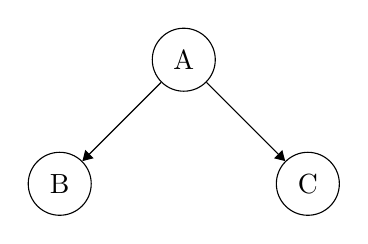
\begin{tikzpicture}[
    node/.style={circle, draw, minimum size=0.8cm},
    -Triangle
]
    \node[node] (A) {A};
    \node[node] (B) [below left=of A] {B};
    \node[node] (C) [below right=of A] {C};
    
    \draw (A) -> (B);
    \draw (A) -> (C);
\end{tikzpicture}
\end{center}

\begin{itemize}
    \item \textbf{用队列:}
    \begin{enumerate}
        \item 初始时,只有A的入度为0。队列:`[A]`。
        \item A出队。序列:`[A]`。B和C的入度都变为0。
        \item 将B和C入队。如果先B后C,队列为`[B, C]`。最终序列为 \textbf{A, B, C}。
        \item 如果先C后B,队列为`[C, B]`。最终序列为 \textbf{A, C, B}。
    \end{enumerate}
    \item \textbf{用栈(DFS):}
    \begin{enumerate}
        \item 从A开始DFS。
        \item 访问A的邻居,如果先访问B,则DFS路径为 A -> B。B没有后代,B完成,B入栈。
        \item 回溯到A,访问另一个邻居C。DFS路径为 A -> C。C没有后代,C完成,C入栈。
        \item 回溯到A,A的所有邻居都已访问,A完成,A入栈。
        \item 栈中内容(从栈顶到栈底):A, C, B。
        \item 依次弹出,得到序列 \textbf{A, C, B}。
    \end{enumerate}
\end{itemize}

在这个例子中,队列可以产生 `A, B, C`,而栈(DFS)可以产生 `A, C, B`。由于可以产生不同的结果,所以答案是“有可能会不同”。
\end{solution}

\section*{173}
\begin{graybox}
若将n个顶点e条弧的有向图采用邻接表存储,
则拓扑排序算法的时间复杂度是:
A. O(n×e)
B. O(n\textsuperscript{2})
C. O(n+e)
D. O(n)
\end{graybox}

\begin{solution}
正确答案是 C。

\textbf{详细分析:}

拓扑排序主要有两种经典的实现算法:基于Kahn算法(入度)和基于DFS。我们来分析这两种算法在使用邻接表存储时的复杂度。

\subsection*{1. 基于Kahn算法(使用队列和入度)}
\begin{enumerate}
    \item \textbf{计算所有顶点的入度:}
    需要遍历整个邻接表一次。遍历所有顶点的邻接表,总共会访问 `n` 个顶点和 `e` 条边。因此,这部分的时间复杂度是 $O(n+e)$。

    \item \textbf{初始化队列:}
    将所有入度为0的顶点入队。这需要扫描所有 `n` 个顶点一次,时间复杂度为 $O(n)$。

    \item \textbf{主循环:}
    循环执行直到队列为空。
    \begin{itemize}
        \item 每个顶点最多入队一次,出队一次。所以对顶点的操作总共是 $O(n)$。
        \item 当一个顶点出队时,会遍历其所有的出边(即其在邻接表中的邻居列表)。在整个算法的生命周期中,每条边都只会被访问一次。所以对边的操作总共是 $O(e)$。
    \end{itemize}
\end{enumerate}
综合以上步骤,Kahn算法的总时间复杂度为 $O(n+e) + O(n) + O(n) + O(e) = O(n+e)$。

\subsection*{2. 基于深度优先搜索(DFS)}
\begin{enumerate}
    \item 拓扑排序可以通过DFS实现:对图进行DFS,当一个顶点完成搜索后(即其所有后代都已被访问),将其加入一个列表的前端(或压入一个栈)。
    \item 对一个用邻接表表示的图进行完整的DFS遍历,需要访问每个顶点和每条边一次。
    \item 因此,DFS本身的时间复杂度就是 $O(n+e)$。
    \item 将顶点加入列表或压栈的操作是 $O(1)$,对所有顶点操作总共是 $O(n)$。
\end{enumerate}
DFS算法的总时间复杂度由DFS遍历主导,因此也是 $O(n+e)$。

\textbf{结论:}
无论使用哪种主流算法,在邻接表存储结构下,拓扑排序的时间复杂度都是 $O(n+e)$。
\end{solution}


\section*{174}
\begin{graybox}
对下图进行拓扑排序,可以得到不同的
拓扑序列的个数是:
\begin{center}
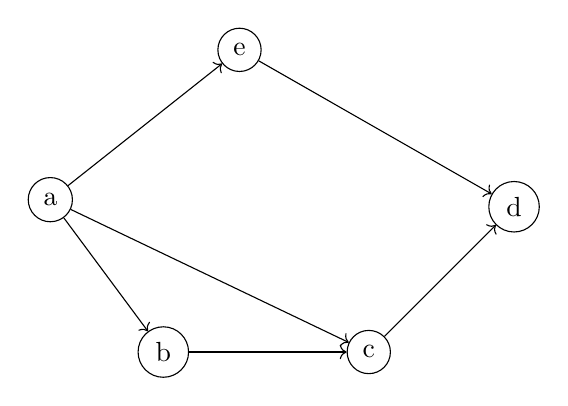
\begin{tikzpicture}[
    node distance=2cm, % Default distance between nodes
    every node/.style={circle, draw}, % Style for all nodes: circular shape, drawn border
    every edge/.style={->, thick} % Style for all edges: arrow at the end, thick line
]

    % Define nodes with relative positioning to each other to mimic the image layout
    \node (a) {a};
    \node (e) [above right=1.5cm and 2cm of a] {e}; % e is above and to the right of a
    \node (b) [below right=1.5cm and 1cm of a] {b}; % b is below and to the right of a
    \node (c) [right=2cm of b] {c}; % c is to the right of b, roughly below e
    \node (d) [above right=2cm of c] {d}; % d is to the right of c, aligning with e-d path

    % Draw the edges (arrows)
    \draw [->] (a) -- (c);
    \draw [->] (a) -- (b);
    \draw [->] (b) -- (c);
    \draw [->] (e) -- (d);
    \draw [->] (c) -- (d);
    \draw [->] (a) -- (e);
\end{tikzpicture}
\end{center}
A. 1\\
B. 2\\
C. 3\\
D. 4
\end{graybox}

\begin{solution}
正确答案是 C。

\textbf{详细分析:}

我们使用Kahn算法(基于入度)来找出所有可能的拓扑序列。

\begin{enumerate}
    \item \textbf{计算初始入度:}
    \begin{itemize}
        \item in(a) = 0
        \item in(b) = 1 (来自 a)
        \item in(c) = 2 (来自 a, b)
        \item in(d) = 2 (来自 e, c)
        \item in(e) = 1 (来自 a)
    \end{itemize}

    \item \textbf{第一步:}
    \begin{itemize}
        \item 只有顶点 \textbf{a} 的入度为0。所以任何拓扑序列都必须以 \textbf{a} 开头。
        \item 序列:`[a]`
        \item “移除” a 和它的出边 (a,b), (a,c), (a,e)。更新邻居的入度:
        \begin{itemize}
            \item in(b) 变为 0
            \item in(c) 变为 1
            \item in(e) 变为 0
        \end{itemize}
    \end{itemize}

    \item \textbf{第二步:}
    \begin{itemize}
        \item 现在入度为0的顶点是 \textbf{b} 和 \textbf{e}。这里出现了分支,我们可以选择先处理b,也可以选择先处理e。
    \end{itemize}

    \item \textbf{分支 1:先选择 b}
    \begin{itemize}
        \item 序列:`[a, b]`
        \item “移除” b 和它的出边 (b,c)。更新邻居的入度:in(c) 变为 0。
        \item 此时,入度为0的顶点是 \textbf{c} 和 \textbf{e}。又出现了一个分支。
        \begin{itemize}
            \item \textbf{分支 1.1:先选择 c}
            \begin{itemize}
                \item 序列:`[a, b, c]`
                \item 移除 c,更新 d 的入度:in(d) 变为 1。
                \item 此时只有 \textbf{e} 的入度为0。
                \item 序列:`[a, b, c, e]`
                \item 移除 e,更新 d 的入度:in(d) 变为 0。
                \item 最后选择 \textbf{d}。
                \item \textbf{得到序列 1:a, b, c, e, d}
            \end{itemize}
            \item \textbf{分支 1.2:先选择 e}
            \begin{itemize}
                \item 序列:`[a, b, e]`
                \item 移除 e,更新 d 的入度:in(d) 变为 1。
                \item 此时只有 \textbf{c} 的入度为0。
                \item 序列:`[a, b, e, c]`
                \item 移除 c,更新 d 的入度:in(d) 变为 0。
                \item 最后选择 \textbf{d}。
                \item \textbf{得到序列 2:a, b, e, c, d}
            \end{itemize}
        \end{itemize}
    \end{itemize}

    \item \textbf{分支 2:先选择 e}
    \begin{itemize}
        \item 序列:`[a, e]`
        \item “移除” e 和它的出边 (e,d)。更新邻居的入度:in(d) 变为 1。
        \item 此时,入度为0的顶点只有 \textbf{b}。没有分支。
        \item 序列:`[a, e, b]`
        \item 移除 b,更新 c 的入度:in(c) 变为 0。
        \item 此时只有 \textbf{c} 的入度为0。
        \item 序列:`[a, e, b, c]`
        \item 移除 c,更新 d 的入度:in(d) 变为 0。
        \item 最后选择 \textbf{d}。
        \item \textbf{得到序列 3:a, e, b, c, d}
    \end{itemize}
\end{enumerate}

综上所述,总共有3个不同的拓扑序列。
\end{solution}


\section*{175}
\begin{graybox}
Prim 算法是通过每步添加一条边及其相连
的顶点到一棵树,从而逐步生成最小生成树。
\end{graybox}

\begin{solution}
这个说法是\textbf{正确}的。

\textbf{详细分析:}

Prim算法是一种用于在加权无向图中寻找最小生成树(MST)的贪心算法。其核心思想可以概括为“加点法”,具体步骤如下:

\begin{enumerate}
    \item \textbf{初始化:}
    \begin{itemize}
        \item 创建一个集合 `U`,用于存放已经在最小生成树中的顶点。
        \item 任意选择一个起始顶点 `s`,将其加入集合 `U`。
        \item 创建一个集合 `T`,用于存放最小生成树的边,初始为空。
    \end{itemize}

    \item \textbf{循环生长:}
    重复以下步骤 `n-1` 次(`n` 是顶点总数):
    \begin{itemize}
        \item 在所有连接集合 `U` 内的顶点与集合 `V-U`(即尚未加入树的顶点)外的顶点的边中,寻找一条权重最小的边 `(u, v)`,其中 `u` $\in$ `U` 且 `v` $\in$ `V-U`。
        \item 将这条权重最小的边 `(u, v)` 加入到集合 `T` 中。
        \item 将顶点 `v` 加入到集合 `U` 中。
    \end{itemize}

    \item \textbf{结束:}
    当所有顶点都加入到集合 `U` 中时,集合 `T` 中的所有边就构成了图的最小生成树。
\end{enumerate}

\textbf{结论:}
这个过程完全符合题目的描述。Prim算法在每一步都选择一条最“划算”的边,将一个新顶点“拉入”到正在构建的树中,从而使这棵树不断“生长”,直到覆盖所有顶点。它始终维护着一个连通的树结构。
\end{solution}


\section*{176}
\begin{graybox}
数据结构中Dijkstra算法用来解决哪个
问题?
A. 字符串匹配
B. 最短路径
C. 拓扑排序
D. 关键路径
\end{graybox}

\begin{solution}
正确答案是 B。

\textbf{详细分析:}

\begin{itemize}
    \item \textbf{B. 最短路径 (Shortest Path):}
    Dijkstra算法是解决\textbf{单源最短路径问题}的经典算法。它用于计算一个加权图中,从一个指定的起始顶点(源点)到所有其他顶点的最短路径。一个关键的限制是,Dijkstra算法要求图中所有的边的权重都必须是\textbf{非负数}。

    \item \textbf{A. 字符串匹配 (String Matching):}
    这是在一段文本中查找一个特定模式串的问题。常用的算法有KMP算法、Boyer-Moore算法等,与图论无关。

    \item \textbf{C. 拓扑排序 (Topological Sort):}
    这是对有向无环图(DAG)的顶点进行线性排序,使得对于每一条有向边 `(u, v)`,`u` 都在 `v` 的前面。常用的算法是Kahn算法或基于DFS的算法。

    \item \textbf{D. 关键路径 (Critical Path):}
    这是在项目管理中,对一个表示工程流程的有向无环图(AOV网)进行分析,找出从开始到结束耗时最长的路径。这条路径就是关键路径。虽然它也涉及路径计算,但它本质上是求解一个\textbf{最长路径}问题,并且是在拓扑排序的基础上进行的,与Dijkstra算法不同。
\end{itemize}
\end{solution}


\section*{177}
\begin{graybox}
若从无向图的任意一个顶点出发进行一次深
度优先搜索可以访问图中所有的顶点,则该图一定
是( )图。
A. 非连通
B. 连通
C. 强连通
D. 有向
\end{graybox}

\begin{solution}
正确答案是 B。

\textbf{详细分析:}

\begin{enumerate}
    \item \textbf{深度优先搜索(DFS)的性质:}
    在任何图(有向或无向)中,从一个顶点 `v` 开始进行一次深度优先搜索,能够访问到的所有顶点集合,恰好是包含顶点 `v` 的那个\textbf{连通分量}中的所有顶点。

    \item \textbf{题目条件分析:}
    题目指出“从\textbf{任意一个顶点}出发进行\textbf{一次}深度优先搜索可以访问图中\textbf{所有的顶点}”。
    \begin{itemize}
        \item “一次”DFS能访问所有顶点,意味着这个图只有一个连通分量。
        \item “从任意一个顶点出发”都成立,这加强了上述结论。
    \end{itemize}

    \item \textbf{连通图的定义:}
    一个无向图被称为\textbf{连通图},如果图中任意两个顶点之间都存在一条路径。这等价于说,这个图只有一个连通分量。

    \item \textbf{结论:}
    题目所描述的性质,正是连通图的定义。因此,该图一定是连通图。
\end{enumerate}

\textbf{其他选项分析:}
\begin{itemize}
    \item \textbf{A. 非连通:} 如果图是非连通的,它至少有两个连通分量。从一个分量的顶点出发,一次DFS无法访问到另一个分量的顶点。
    \item \textbf{C. 强连通:} “强连通”是\textbf{有向图}的概念,指图中任意两个顶点之间都互相可达。对于无向图,其对应的概念就是“连通”。
    \item \textbf{D. 有向:} 题目明确说明是“无向图”。
\end{itemize}
\end{solution}

\section*{178}
\begin{graybox}
使用Dijkstra算法求下图中从顶点1到其
他各顶点的最短路径,依次得到的各最短路径的目标顶点是:
\begin{center}
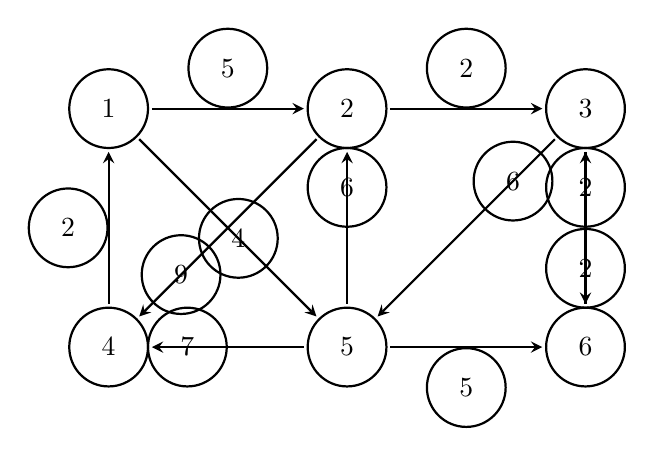
\begin{tikzpicture}[
    node distance=2cm,
    every node/.style={circle, draw, thick, minimum size=1cm},
    every edge/.style={draw, thick, -stealth, shorten >=1pt, shorten <=1pt}
]

% Nodes
\node (1) {1};
\node (2) [right=of 1] {2};
\node (3) [right=of 2] {3};
\node (4) [below=of 1] {4};
\node (5) [below=of 2] {5};
\node (6) [below=of 3] {6};

% Edges
\path (1) edge node[above] {5} (2);
\path (1) edge node[pos=0.4, below right] {4} (5);
\path (2) edge node[above] {2} (3);
\path (2) edge node[pos=0.6, below left] {9} (4);
\path (3) edge node[pos=0.4, above right] {6} (5);
\path (3) edge node[below] {2} (6);
\path (4) edge node[left] {2} (1);
\path (5) edge node[left] {7} (4);
\path (5) edge node[below] {5} (6);
\path (5) edge node[above] {6} (2);
\path (6) edge node[above] {2} (3);

\end{tikzpicture}
\end{center}
A. 5, 2, 6, 3, 4\\
B. 5, 2, 3, 6, 4\\
C. 5, 2, 4, 3, 6\\
D. 5, 2, 3, 4, 6
\end{graybox}

\begin{solution}
正确答案是 B。

\textbf{详细分析:}

Dijkstra算法的步骤如下:
\begin{itemize}
    \item `S`: 已找到最短路径的顶点集合。
    \item `dist[v]`: 从源点1到顶点v的当前最短路径长度。
\end{itemize}

我们用一个表格来追踪算法的执行过程。

\begin{table}[h!]
\centering
\begin{tabular}{|c|l|l|c|}
\hline
\textbf{步骤} & \textbf{S (已确定集合)} & \textbf{dist 数组 (对未确定顶点)} & \textbf{选定顶点} \\ \hline
\textbf{初始} & \{1\} & dist[2]=5, dist[4]=$\infty$, dist[5]=4, dist[3,6]=$\infty$ & - \\ \hline
\textbf{1} & \{1, \textbf{5}\} & dist[2]=5, dist[4]=11, dist[6]=9, dist[3]=$\infty$ & \textbf{5} (dist=4) \\ \hline
\textbf{2} & \{1, 5, \textbf{2}\} & dist[4]=11, dist[6]=9, dist[3]=7 & \textbf{2} (dist=5) \\ \hline
\textbf{3} & \{1, 5, 2, \textbf{3}\} & dist[4]=11, dist[6]=9 & \textbf{3} (dist=7) \\ \hline
\textbf{4} & \{1, 5, 2, 3, \textbf{6}\} & dist[4]=11 & \textbf{6} (dist=9) \\ \hline
\textbf{5} & \{1, 5, 2, 3, 6, \textbf{4}\} & - & \textbf{4} (dist=11) \\ \hline
\end{tabular}
\end{table}

\textbf{过程分解:}
\begin{enumerate}
    \item \textbf{初始化:} `S = {1}`。`dist[1]=0`。1的邻居是2和5,所以 `dist[2]=5`, `dist[5]=4`。
    \item \textbf{第1轮:}
    \begin{itemize}
        \item 在未确定的顶点中,5的距离最短(`dist[5]=4`)。将 \textbf{5} 加入 `S`。
        \item 更新5的邻居:
        \begin{itemize}
            \item 到2: `dist[5]+d(5,2) = 4+6=10` > `dist[2]=5`,不更新。
            \item 到4: `dist[5]+d(5,4) = 4+7=11`。更新 `dist[4]=11`。
            \item 到6: `dist[5]+d(5,6) = 4+5=9`。更新 `dist[6]=9`。
        \end{itemize}
    \end{itemize}
    \item \textbf{第2轮:}
    \begin{itemize}
        \item 在未确定的顶点 {2,3,4,6} 中,2的距离最短(`dist[2]=5`)。将 \textbf{2} 加入 `S`。
        \item 更新2的邻居:
        \begin{itemize}
            \item 到3: `dist[2]+d(2,3) = 5+2=7`。更新 `dist[3]=7`。
            \item 到4: `dist[2]+d(2,4) = 5+9=14` > `dist[4]=11`,不更新。
        \end{itemize}
    \end{itemize}
    \item \textbf{第3轮:}
    \begin{itemize}
        \item 在未确定的顶点 {3,4,6} 中,3的距离最短(`dist[3]=7`)。将 \textbf{3} 加入 `S`。
        \item 更新3的邻居:
        \begin{itemize}
            \item 到6: `dist[3]+d(3,6) = 7+2=9` = `dist[6]=9`,不更新。
        \end{itemize}
    \end{itemize}
    \item \textbf{第4轮:}
    \begin{itemize}
        \item 在未确定的顶点 {4,6} 中,6的距离最短(`dist[6]=9`)。将 \textbf{6} 加入 `S`。
        \item 6的邻居3已在S中,无更新。
    \end{itemize}
    \item \textbf{第5轮:}
    \begin{itemize}
        \item 只剩下顶点4。将 \textbf{4} 加入 `S`。
    \end{itemize}
\end{enumerate}

算法依次找到最短路径的目标顶点顺序为:\textbf{5, 2, 3, 6, 4}。
\end{solution}


\section*{179}
\begin{graybox}
Dijkstra算法是按路径长度递增的顺序依次产生从某一固定源点到其他各顶点之间的最短路径。
\end{graybox}

\begin{solution}
这个说法是\textbf{正确}的。

\textbf{详细分析:}

Dijkstra算法的本质是一个贪心算法。它维护两个顶点集合:
\begin{itemize}
    \item \textbf{S}: 已经找到从源点出发的最短路径的顶点集合。
    \item \textbf{V-S}: 尚未找到从源点出发的最短路径的顶点集合。
\end{itemize}

算法的核心步骤如下:
\begin{enumerate}
    \item 初始化:`S` 中只包含源点 `s`。
    \item 循环执行:在每一步中,算法从集合 `V-S` 中选择一个顶点 `u`,该顶点 `u` 满足一个条件:从源点 `s` 到 `u` 的当前已知路径长度是所有 `V-S` 中顶点里最短的。
    \item 更新:将选出的顶点 `u` 从 `V-S` 移动到 `S` 中。此时,可以断定从 `s` 到 `u` 的这条路径就是最终的最短路径。
    \item 松弛:更新 `u` 的所有邻居的路径信息。
\end{enumerate}

\textbf{关键点在于第2步的贪心选择}:算法总是选择当前看起来“最近”的顶点进行处理。由于图中没有负权边,这个贪心选择是正确的。当一个顶点 `u` 被选中并加入集合 `S` 时,它的最短路径长度就已经确定了。因为算法总是选择路径长度最小的顶点,所以被加入到 `S` 的顶点序列,其对应的最短路径长度必然是\textbf{非递减}(即递增或相等)的。

因此,Dijkstra算法确实是按照路径长度递增的顺序,一步步地确定从源点到其他各顶点的最短路径。
\end{solution}


\section*{180}
\begin{graybox}
在对有向无环图执行拓扑排序算法之后,
入度数组中所有元素的值均为0。
\end{graybox}

\begin{solution}
这个说法是\textbf{正确}的。

\textbf{详细分析:}

我们以基于入度的Kahn算法为例来分析拓扑排序的过程:

\begin{enumerate}
    \item \textbf{初始化:}
    算法开始时,会计算图中每个顶点的初始入度,并存储在一个入度数组 `in\_degree` 中。

    \item \textbf{算法核心循环:}
    \begin{itemize}
        \item 算法将所有初始入度为0的顶点放入一个队列(或栈)中。
        \item 接着,算法从队列中取出一个顶点 `u`,并将其加入到拓扑序列中。
        \item 对于顶点 `u` 的每一个邻接点 `v`(即存在边 `<u, v>`),算法会将 `v` 的入度减1(`in\_degree[v]--`)。这个操作可以理解为在逻辑上“删除”了边 `<u, v>`。
        \item 如果 `v` 的入度在减1后变为0,就将 `v` 加入队列。
    \end{itemize}

    \item \textbf{算法结束条件:}
    对于一个有向无环图(DAG),这个过程会持续进行,直到图中所有的顶点都被加入到拓扑序列中。

    \item \textbf{最终状态:}
    \begin{itemize}
        \item 当算法成功结束时,意味着图中的每一条边 `<u, v>` 都被“删除”了一次。
        \item 每删除一条边 `<u, v>`,顶点 `v` 的入度就会减1。
        \item 既然所有的边都被删除了,那么每个顶点的入度都从其初始值减少了相应的值,最终必然会归零。
    \end{itemize}
\end{enumerate}

\textbf{结论:}
拓扑排序算法的执行过程,在逻辑上等同于不断地移除图中的边,直到图变为空图(没有边)。当算法完成时,所有顶点的入度自然都变为了0。
\end{solution}










\end{document}

% VScode 常用快捷键:

% Ctrl + R:                 打开最近的文件夹
% F2:                       变量重命名
% Ctrl + Enter:             行中换行
% Alt + up/down:            上下移行
% 鼠标中键 + 移动:           快速多光标
% Shift + Alt + up/down:    上下复制
% Ctrl + left/right:        左右跳单词
% Ctrl + Backspace/Delete:  左右删单词    
% Shift + Delete:           删除此行
% Ctrl + J:                 打开 VScode 下栏(输出栏)
% Ctrl + B:                 打开 VScode 左栏(目录栏)
% Ctrl + `:                 打开 VScode 终端栏
% Ctrl + 0:                 定位文件
% Ctrl + Tab:               切换已打开的文件(切标签)
% Ctrl + Shift + P:         打开全局命令(设置)

% Latex 常用快捷键

% Ctrl + Alt + J:           由代码定位到PDF
% 


% Git提交规范:
% update: Linear Algebra 2 notes
% add: Linear Algebra 2 notes
% import: Linear Algebra 2 notes
% delete: Linear Algebra 2 notes
